\documentclass[thesis.tex]{subfiles}
\begin{document}
\chapter{Applying AppPAL to BYOD policies}
\label{chap:byod}

Many employees bring their personal mobile devices to work. To control
the access these devices have to company resources, an estimated 72\%
of companies publish \ac{BYOD} policies.\footnote{According to survey
  of companies by LinkedIn~\cite{schulze_byod_2016}. 40\% made \ac{BYOD}
  available to all employees, 32\% made it available to select
  employees.} These \ac{BYOD} policies are natural language documents
that employees should read and obey. They describe steps to take to
secure devices in the workplace. The policies say how employees should
get access to data, and who should authorise decisions.

Companies can use their policies in varying ways. Some companies may
trust employees to follow the rules on their own. Alternatively
\ac{MDM} software can implement part of the policies: packages such as
IBM's MaaS360 and Blackberry's BES~\cite{ibm_ibm_nodate,blackberry_secure_nodate} can
configure devices to restrict functionality and manage apps.

Commercial tools have limits to what they currently enforce. Some
tools can only enable simple on-off configuration settings, and ban
explicitly black-listed apps. More advanced systems can use
app-rewriting to recompile apps to tunnel traffic through a VPN, or
geofencing to apply policies in predefined areas. These tools are not
infallible. One survey found that 50\% of companies with \ac{MDM}
software still had non-compliant devices in their
networks~\cite{mobileiron_security_labs_q4_2015}. Whilst app wrapping
can protect some apps, in general it is
ineffective~\cite{hao_effectiveness_2013}.

\section{Overview of five BYOD policies}
\label{sec:overview-of-five-byod-policies}

Through out this chapter, we will explore how we can apply AppPAL to
BYOD policies through the analysis of five \emph{real-world} policies.
We chose the policies from a variety of domains.  They cover a range
of different policy styles and concerns.  Two are example policy
templates a company might want to base its own BYOD policy on,
published by security advice organizations.  The remaining three are
BYOD policies used inside companies.

\begin{enumerate}
\item Is the \emph{Security Policy Template: Use of Handheld Devices
    in a Corporate Environment}, published by the SANS
  Institute~\cite{nicholas_r._c._guerin_security_2008}. This policy is a
  hypothetical policy published to help companies mitigate the threats
  to corporate assets caused by mobile devices. Companies change the
  document to suit their needs and BYOD requirements. The policy is
  general; not specific to any particular industry, device, or country's
  legislation.
\item Is from a US non-profit company trying to improve health care through IT, called \ac{HiMSS} \cite{healthcare_information_and_management_systems_society_mobile_2012}. The
  \ac{HiMSS} policy is relatively short and has concerns specific to
  healthcare scenarios. The policy is a contract the users follow. The
  police has a different style to other policies: in the other policies
  the company states what users should do, here the user states what
  they will do.  The policy is designed as a sample agreement for a
  system trying to manage personal mobile devices in a healthcare
  environment.
\item Is from a British hospital trust~\cite{kennington_mobiles_2014}
  and describes the BYOD scheme used in practice at the hospital.  The
  policy is broad and covers rules for corporately owned devices.  This
  policy also briefly describes how devices should interact with
  patients.
\item Is a relatively simple policy from The University of
  Edinburgh~\cite{williamson_bring_2015}. It is briefer, and groups
  rules into sections for high and low risk users, unlike the other
  policies.  The policy is extremely general describing rules for
  laptops, tablets and phones.  Many of the rules are vague.
  The policy says \emph{``Use anti-virus software and keep it up
    to date''}, leaving the choice of AV software, and
  update times to the user.
\item Is by a company specialising in emergency
  sirens~\cite{code3pse.org_sample_nodate}. Again this policy is simpler,
  and like the Edinburgh policy rather general compared to the other policies.
\end{enumerate}

Each of the policies is split into a series of rules and requirements employees
should follow. Typically the policy is describing what employees should
do and what will happen under certain circumstances. For example the NHS policy
states that:

\begin{policyrule}{NHS}
  In the event of loss of the device, all data including apps will be wiped. The Trust
  is not responsible for reimbursement of any costs for personally purchased apps.
\end{policyrule}

The Siren policy matches this style, stating what conditions will lead to the
company wiping an employees device:

\begin{policyrule}{Sirens}
The employee's device may be remotely wiped if: $\bullet$ The device is lost or
stolen. $\bullet$ The employee terminates his or her employment. $\bullet$ IT
detects a data or policy breach, a virus or similar threat to the security of
the company's data and technology infrastructure.
\end{policyrule}

As mentioned before the \ac{HiMSS} policy has a different style.  This is shown
by the equivalent rule being phrased from the perspective of the policy subject
(\emph{``I agree\dots''}).

\begin{policyrule}{HiMSS}
  I agree that the PDA/Smartphone can be wiped by XYZ Health System upon the
  decision of XYZ Health System management and understand that it will delete all
  data including personal files.
\end{policyrule}

The SANS policy is mostly written in the same style as the NHS policy.  It is
proposed as a template policy that a company might use as the basis for their
own policy, however it sometimes says things that seem like advice to an IT
department implementing the policy.  For example:

\begin{policyrule}{SANS}
   A corporate mobile device management solution SHALL feature remote device
   wiping (or possibly only blocking) mechanism for all devices accessing
   corporate internal networks.
\end{policyrule}

The SANS policy also distinguishes between rules that should always be followed (SHALL),
and those that may depend on a specific business's situation (SHOULD).

\begin{policyrule}{SANS}
  Basically, sentences using the verb ``SHALL'' are mandatory requirements
  applying to practices with high probability of putting the business at risk,
  whereas ``SHOULD'' means that the policy needs to be applied according to the
  business's specific situation.
\end{policyrule}

The Edinburgh policy takes this even further. The policy groups rules by device type
and gives a security level.  The policy expects high and medium risk users
to follow everything, and low risk users to at least
consider following the rules marked with a $\nabla$.  For example the policy groups together the
rule for remote wiping devices with the rules specific to mobile
devices and tablets. 

\begin{policyrule}{Edinburgh}
  $\nabla$ Configure your device to enable you to remote-wipe it should it become lost.
\end{policyrule}

We present a version of each policy that presents the policy text
alongside the AppPAL translation in \autoref{appendix:byod}.  The
remainder of this chapter looks at what we discovered from the
translation process, and comments on \ac{MDM} policies in general.

\section{Review of MDM software}

A company might use \ac{MDM} software to enforce their rules.  Many
companies offer an \ac{MDM} solutions, including IBM (with their tool
\emph{MaaS360}), VMware (\emph{AirWatch}) and MobileIron (whose tool
has the same name as the company). They offer a comparable set of
features, namely:
\begin{enumerate}
\item App wrapping; where an app is modified to offer some additional
  features or network properties. This is often limited to routing all
  the app's network traffic through a VPN.
\item Basic security configuration; allows an administrator to turn on
  and off various device settings and security features. This might
  include wifi settings, passcodes, encryption and Bluetooth.  These
  features could be used to reduce the attack surface of a device by
  disabling features, or enforce policies that require a user's location
  to always be accessible by turning on the GPS.
\item Provisioning; where IT departments can install and update apps and
  their configuration files. Email and LDAP configuration is common.
\item A curated app store; where IT departments can white-or-black-list apps.
\end{enumerate}

The features of 9 competing \ac{MDM} packages identified by a Gartner
report are summarised in
\autoref{tab:mdm-capabilities}~\cite{rob_smith_magic_2016}.  Most of
the tools link to the report on their homepages as the report lists
\emph{every} tool as either \emph{visionary}, \emph{leading}, or
\emph{niche player}, though the precise differences between them is unclear.\footnote{Table~\ref{tab:mdm-capabilities}
  summarises the visionary and leading \ac{MDM} packages.}  The tools are very similar with the chief difference being the UI
as well as some extra features only certain tools support.

\begin{table}\centering\sffamily\footnotesize
  \begin{tabular}{l c c c c c c c c c}
    \toprule
    Feature                           & \rb{MaaS360} & \rb{Blackberry BES} & \rb{MobileIron} & \rb{Citrix XenMobile} & \rb{VMWare AirWatch} & \rb{Microsoft} & \rb{SOTI MobiControl} & \rb{Sophos} & \rb{Landdesk} \\
    \midrule
    Antivirus                         &              &                     &                 &                       &                      &                &                       & \cmark      &               \\
    App selection/store/management    & \cmark       & \cmark              & \cmark          & \cmark                & \cmark               & \cmark         & \cmark                & \cmark      & \cmark        \\
    App wrapping/modification         &              & \cmark              & \cmark          & \cmark                & \cmark               & \cmark         &                       & \cmark      & \cmark        \\
    Authentication                    & \cmark       & \cmark              & \cmark          & \cmark                & \cmark               & \cmark         & \cmark                &             &               \\
    Compliance reporting              & \cmark       & \cmark              & \cmark          & \cmark                & \cmark               & \cmark         & \cmark                & \cmark      &               \\
    Device configuration              & \cmark       & \cmark              & \cmark          & \cmark                & \cmark               & \cmark         & \cmark                &             & \cmark        \\
    Email/Calendar/Contacts/Documents & \cmark       & \cmark              & \cmark          & \cmark                & \cmark               & \cmark         & \cmark                & \cmark      & \cmark        \\
    Feature Restrictions              & \cmark       & \cmark              &                 &                       & \cmark               & \cmark         &                       &             &               \\
    Licence distribution              &              & \cmark              &                 &                       &                      &                &                       &             &               \\
    Location based settings           & \cmark       &                     &                 &                       & \cmark               &                &                       &             &               \\
    Network configuration             & \cmark       & \cmark              & \cmark          & \cmark                & \cmark               & \cmark         & \cmark                &             &               \\
    Password/Encryption settings      & \cmark       & \cmark              & \cmark          & \cmark                & \cmark               & \cmark         & \cmark                & \cmark      &               \\
    Remote wipe                       & \cmark       & \cmark              & \cmark          & \cmark                & \cmark               & \cmark         & \cmark                & \cmark      & \cmark        \\
    Security auditing                 & \cmark       & \cmark              & \cmark          & \cmark                & \cmark               & \cmark         & \cmark                & \cmark      &               \\
    Tracking/Spyware                  & \cmark       & \cmark              &                 &                       &                      & \cmark         & \cmark                &             & \cmark        \\
    Watermarking                      &              &                     &                 &                       & \cmark               &                &                       &             &               \\
    \bottomrule
  \end{tabular}
  \caption[Summary of different \ac{MDM} capabilities]{%
    Summary of different \ac{MDM} software's capabilities built from information from
    each of the tools sales pages.
  }
  \label{tab:mdm-capabilities}
\end{table}

Whilst \ac{MDM} tools can configure devices, the policies they enforce are less
sophisticated than what you can write with a policy language such as AppPAL. The
policies of an \ac{MDM} tool are essentially granular checkboxes (as shown in
\autoref{fig:maas360-policy}) an administrator can manually enable or disable to
configure a device for a group of users.

\begin{figure}
  \centering
  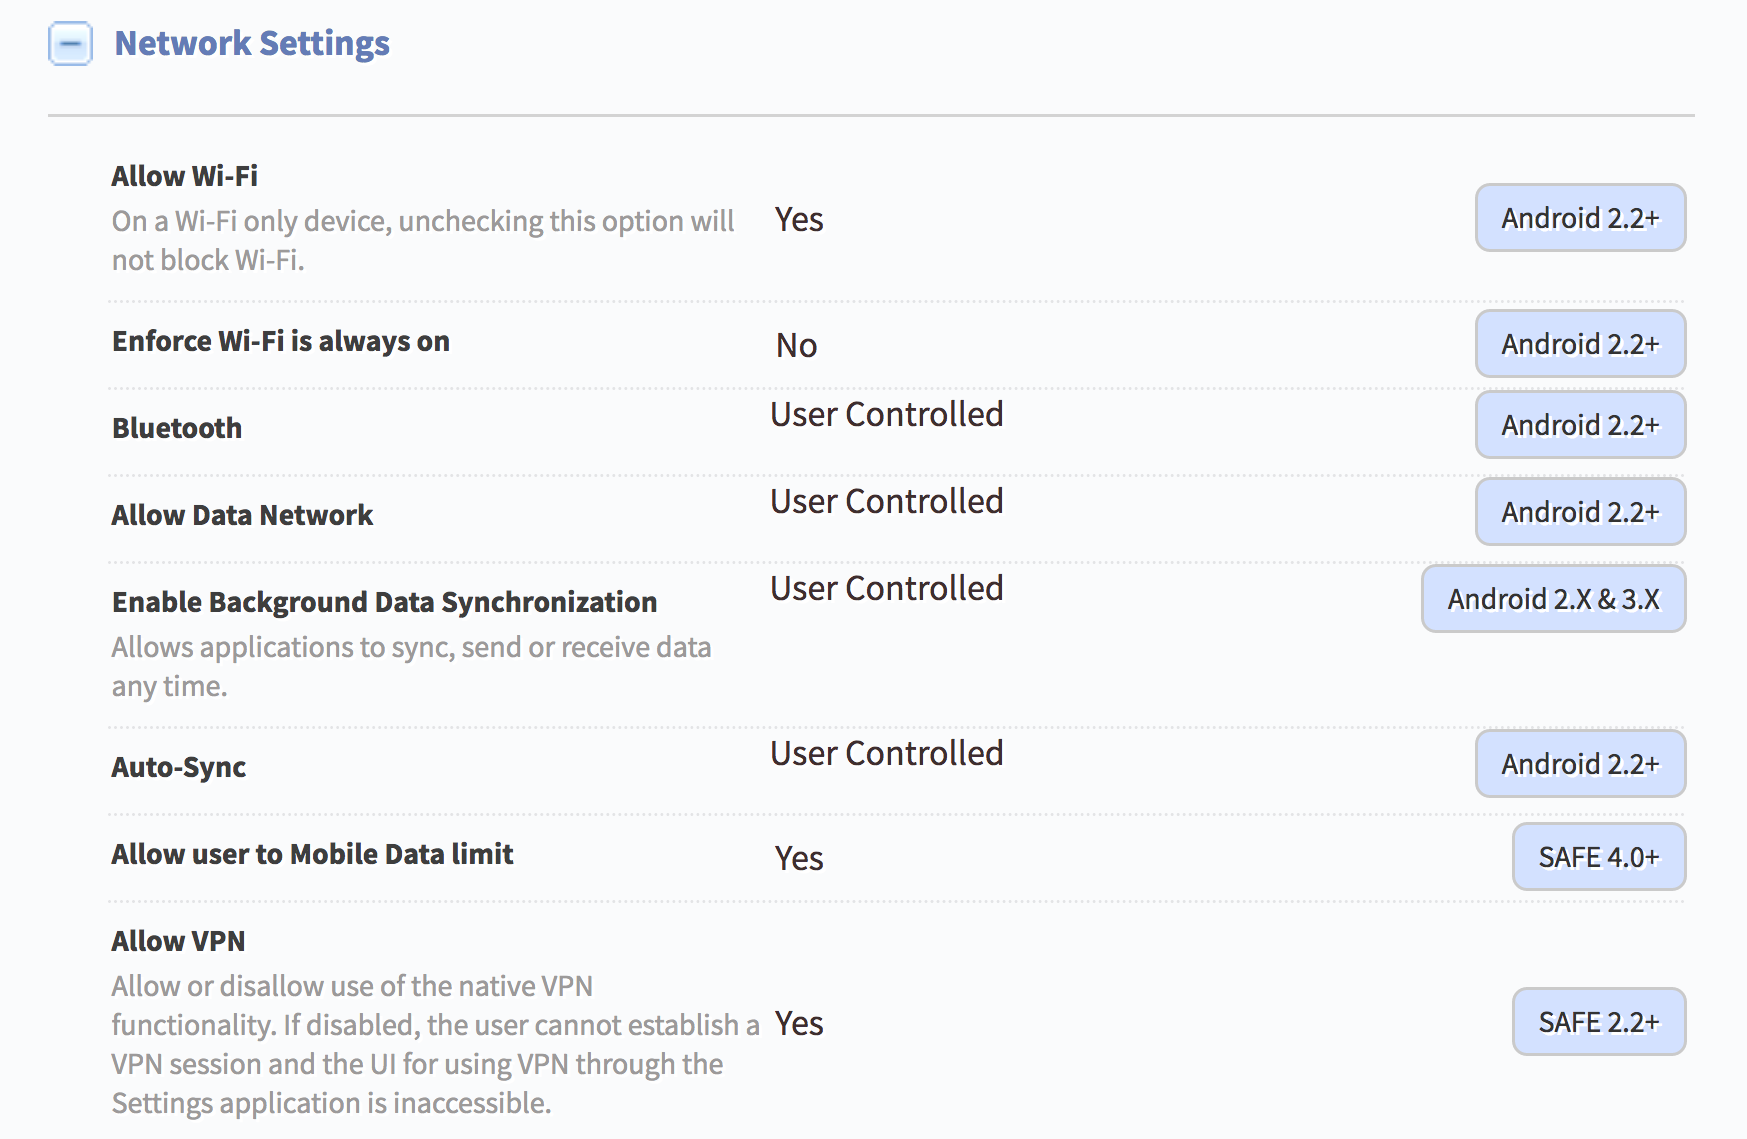
\includegraphics[width=\textwidth]{figures/maas360-policy.png}
  \caption{Policy settings in the MaaS360 \ac{MDM} tool.}
  \label{fig:maas360-policy}
\end{figure}

\subsection{Related BYOD Work}

As well as commercial \ac{MDM} products there are also research tools
that are similar to \ac{MDM} software. Martinelli~\etal{}'s work
creates a dynamic permissions manager, called UC-Droid. Their tool can
alter what an app's Android permissions are at run time, based on
policies~\cite{martinelli_enhancing_2016}.  The tool allows companies
to reconfigure their apps depending on whether the employee is at
work, in a secret lab, or working out-of-hours. These kinds of
policies are more configurable than the geofenced based policies some
\ac{MDM} tools offer. Other work has looked at enforcing different
policies based on what roles an employee
holds~\cite{costantino_towards_2013}. The work allowed a company to
verify the devices within their network and what servers and services
they could reach. It also describes a mechanism for providing
different users with different policies.

Armando~\etal~developed BYODroid as a tool for enforcing BYOD policies through a
secure marketplace~\cite{armando_bring_2013}. Their tool allows companies to
distribute apps through a secure app~store~\cite{armando_enabling_2014}. The
store ensures apps meet policies through a static analysis and
app rewriting to add dynamic enforcement. Their policies are low-level, based on
ConSpec~\cite{aktug_conspec_2008}, allowing checks based on Dalvik VM's state.
Using their tool, they implemented the parts of a NATO Communications and
Information Agency policy about personal networks and data
management~\cite{armando_developing_2016}. Their work shows how to check and enforce the app-specific
sections of a BYOD policy using tools. They did not
look at where the checks or policies come from, however.


\section{Modelling BYOD policies}

Because the policies are written using natural language, which can be ambiguous.
Comparing policies written in different styles from different sources is tricky as the relationships between different entities, and the exact decisions being made can become confused.
To make comparisons precisely we first model the natural language policy's rules in a formal language, namely AppPAL.
We take care to use the same predicates between different policies to create a standard set of decisions between \ac{BYOD} policies.

Each of the policies are split into a series of rules. A simple example is the
following example from the Sirens-company policy. The rule states that devices
may get access to various company resources.
For each resource we create an AppPAL
assertion that states that a device may access the resource.

\begin{policyrule}{Sirens}
  Employees may use their mobile device to access the following company-owned resources:
  \newline $\bullet$ Email $\bullet$ Calendars $\bullet$ Contacts $\bullet$ Documents $\bullet$ Etc.
  \normalfont
  \begin{lstlisting}
'department' says Device:D canAccess('email').
'department' says Device:D canAccess('calendars').
'department' says Device:D canAccess('contacts').
'department' says Device:D canAccess('documents').
  \end{lstlisting}
\end{policyrule}

The NHS policy has a more complex example. Employees are not
allowed to call non-domestic, or premium rate numbers on company-owned
phones , however an employee's manager can make an exception.
To write the AppPAL version of this rule we initially have the default
rule that bans international calls, then we add a second rule stating that it is
allowed if someone makes an exemption, finally a third rule states that an employee's manager 
can make the exemption.

\begin{policyrule}{NHS}
  All mobile devices will be configured for national access only. Premium/international calls will be barred.
  International call barring and roaming arrangements can be lifted for specific periods, to be stipulated on request, on approval of the relevant manager/budget holder.
  \normalfont
  \begin{lstlisting}
'nhs-trust' says Device canCall(TelephoneNumber:X)
  if Device isOwnedBy('nhs-trust'),
     X isNationalNumber, X isStandardRateNumber.

'nhs-trust' says Device canCall(TelephoneNumber:X)
  if Device isOwnedBy(Staff),
     Staff hasCallExemption.

'nhs-trust' says Manager can-say
  Staff hasCallExemption
  if Manager isManagerOf(Staff).
  \end{lstlisting}
\end{policyrule}

Table~\ref{tab:prefix} shows a count of the different types of
predicate used in the policies.  As before in \autoref{chap:apppal}
predicates, we use common prefixes to distinguish different kinds of
predicate.  The use of each is also split by whether the predicate is
a \emph{decision} made by the policy, or a \emph{condition} for making
that decision. \emph{Can} and \emph{must} decisions feature in all
policies excepting \emph{can} decisions in the Edinburgh policy, in
part due to the structure of the policy as discussed in
\autoref{sec:overview-of-five-byod-policies}. We would expect this: these are access
control decisions and reactions to events both topics that existing
\ac{MDM} tools have focused on implementing. \emph{Has} and \emph{is}
predicates are often used in the conditions, but there are also
decisions using them too.

\section{BYOD idioms in AppPAL}
\label{sec:common_concerns}

When examining the policies, there are some concern concerns shared
between the different policies A summary of predicates, with the same
meaning, used in multiple policies by our translation is given in
\autoref{tab:common}.  The table lists predicates (and arguments)
found in multiple policies and indicates which policies they occurred
in.  From it we can look for common interests between policies, and
identify what decisions \ac{BYOD} policies are concerned with.

Acknowledgements, where the policy requests people acknowledge other
policies, and predicates linking devices to owners feature in all
policies.  Most policies describe rules for when to enable and disable
device features.  Configuring device features is a common feature to
many \ac{MDM} packages, but tracking what a user agrees to is not seen
in leading \ac{MDM} packages like MaaS360 or
BES~\cite{rob_smith_magic_2016}.  Only two of the five policies had
rules limiting access to networks, servers, or access points. This is
surprising as a common feature of \ac{MDM} tools is controlling how
devices and apps access networks.  Users have privacy preferences
about apps~\cite{lin_modeling_2014}, but not all companies try to
control what apps employees install.  Providing curated app stores and
blacklisting apps is a feature common to many \ac{MDM} programs.  Not
all policies express rules about which apps to install, however.  All
policies talked about remotely wiping a device for security reasons
(as shown in~\autoref{sec:overview-of-five-byod-policies}); and most
\ac{MDM} programs implemented this by allowing an administrator
remotely erase a device~(\autoref{tab:mdm-capabilities}).

Two particular idioms occur in many policies: acknowledgements and
delegation.  We describe both idioms in greater detail, and show how
to describe them in AppPAL, below.  MDM tools and research have
focussed so far on implementing restrictions on apps and
devices~\cite{ibm_ibm_nodate,armando_formal_2014,martinelli_enhancing_2016}.
Implementing these controls is a vital aspect of BYOD policies and all
5 of the policies we looked at had rules that described
restrictions~(\autoref{tab:common}).  Every policy also contained
rules that required employees acknowledgements, however.  Only the
SANS policy (which is configuration focussed) contained more rules
that required restrictions than acknowledgements.  All the policies
contained more rules featuring delegation relationships than
functionality restrictions.  Restricting device functionality is
tricky and important, but other aspects of BYOD policies are also
worth attention.

\begin{table}\sffamily\small\centering
  \newcommand{\zilch}[0]{\small 0}
  \newcommand{\numpc}[2]{\small #2\% {\small(#2)}}
  \setlength{\tabcolsep}{1pt}
\begin{tabular}{ c  c c c c c c c c c }
\toprule
             & \multicolumn{4}{c}{Decision}                                                    && \multicolumn{4}{c}{Condition} \\
Policy       & \rb{Can}                     & \rb{Must}      & \rb{Has}       & \rb{Is}        && \rb{Can}      & \rb{Must}     & \rb{Has}        & \rb{Is}        \\
\midrule
SANS         & \numpc{26}{35}               & \numpc{22}{29} & \numpc{8 }{9 } & \numpc{20}{27} && \numpc{2 }{2} & \numpc{2 }{2} & \numpc{9 }{8}   & \numpc{82}{87} \\
HiMSS        & \numpc{6 }{21}               & \numpc{12}{41} & \numpc{9 }{31} & \numpc{2 }{7 } && \zilch        & \zilch        & \numpc{3 }{13}  & \numpc{20}{87} \\
NHS          & \numpc{13}{19}               & \numpc{18}{26} & \numpc{23}{33} & \numpc{16}{23} && \numpc{2 }{2} & \zilch        & \numpc{20}{19}  & \numpc{83}{83} \\
Sirens       & \numpc{12}{27}               & \numpc{20}{45} & \numpc{5 }{11} & \numpc{7 }{16} && \numpc{1 }{2} & \numpc{4 }{7} & \numpc{1 }{2}   & \numpc{50}{89} \\
Edinburgh    & \zilch                       & \numpc{3 }{18} & \numpc{9 }{82} & \zilch         && \numpc{2 }{7} & \numpc{2 }{7} & \numpc{15}{ 50} & \numpc{13}{37} \\
\bottomrule \\
\end{tabular}
\caption{Counts of predicate-types in each policy.}
\label{tab:prefix}
\end{table}

\begin{table}\sffamily\footnotesize\centering
  \newcommand{\expred}[3]{\textit{#2} #1\textit{#3}}
  \begin{tabular}{c c c c c c}
    \toprule                                                                                                           \\
    Predicate                                       & \rb{SANS} & \rb{HiMSS} & \rb{NHS} & \rb{Sirens} & \rb{Edinburgh} \\
    \midrule
    \expred{mustAcknowledge}{person}{(policy)}      & \cmark    & \cmark     & \cmark   & \cmark      & \cmark         \\
    \expred{hasAcknowledged}{person}{(policy)}      & \cmark    & \cmark     & \cmark   & \cmark      & \cmark         \\
    \expred{isOwnedBy}{device}{(person)}            & \cmark    & \cmark     & \cmark   & \cmark      & \cmark         \\
    \expred{isDevice}{thing}{}                      & \cmark    & \cmark     & \cmark   & \cmark      & \cmark         \\
    \expred{mustDisable}{device}{(feature)}         & \cmark    &            & \cmark   & \cmark      & \cmark         \\
    \expred{mustWipe}{device}{}                     &           & \cmark     & \cmark   & \cmark      & \cmark         \\
    \expred{isLost}{device}{}                       & \cmark    & \cmark     & \cmark   & \cmark      &                \\
    \expred{isEmployee}{thing}{}                    & \cmark    &            & \cmark   & \cmark      & \cmark         \\
    \expred{isApp}{thing}{}                         & \cmark    & \cmark     & \cmark   & \cmark      &                \\
    \expred{isActivated}{device}{}                  & \cmark    & \cmark     & \cmark   &             & \cmark         \\
    \expred{mustEnable}{device}{(feature)}          & \cmark    & \cmark     &          & \cmark      &                \\
    \expred{isEncrypted}{device}{}                  & \cmark    &            & \cmark   &             & \cmark         \\
    \expred{hasFeature}{device}{(feature)}          & \cmark    &            & \cmark   &             & \cmark         \\
    \expred{hasMet}{device}{(policy)}               & \cmark    &            & \cmark   &             & \cmark         \\
    \expred{canMonitor}{person}{(device)}           & \cmark    &            & \cmark   & \cmark      &                \\
    \expred{mustInform}{person}{(person)}           & \cmark    &            & \cmark   &             &                \\
    \expred{isTelephoneNumber}{thing}{}             & \cmark    &            & \cmark   &             &                \\
    \expred{isString}{thing}{}                      &           &            & \cmark   & \cmark      &                \\
    \expred{isSecurityLevel}{thing}{}               & \cmark    & \cmark     &          &             &                \\
    \expred{isInstallable}{app}{}                   & \cmark    &            & \cmark   &             &                \\
    \expred{isFeature}{thing}{}                     & \cmark    &            &          & \cmark      &                \\
    \expred{isData}{thing}{}                        & \cmark    &            &          & \cmark      &                \\
    \expred{isApprovedFor}{application}{(person)}   &           & \cmark     & \cmark   &             &                \\
    \expred{isApproved}{application}{}              & \cmark    & \cmark     &          &             &                \\
    \expred{hasDevice}{person}{(device)}            &           & \cmark     & \cmark   &             &                \\
    \expred{hasDepartment}{person}{(department)}    &           & \cmark     &          &             & \cmark         \\
    \expred{canUse}{person}{(device)}               & \cmark    &            & \cmark   &             &                \\
    \expred{canStore}{device}{(file)}               & \cmark    & \cmark     &          &             &                \\
    \expred{canInstall}{device}{(app)}              & \cmark    &            & \cmark   &             &                \\
    \expred{canConnectToServer}{device}{(server)}   & \cmark    &            & \cmark   &             &                \\
    \expred{canConnectToNetwork}{device}{(network)} & \cmark    &            &          & \cmark      &                \\
    \expred{canConnectToAP}{device}{(access-point)} & \cmark    & \cmark     &          &             &                \\
    \expred{canCall}{device}{(number)}              & \cmark    &            & \cmark   &             &                \\
    \expred{canBackupTo}{device}{(server)}          &           & \cmark     &          &             & \cmark         \\
    \bottomrule                                                                                                        \\
  \end{tabular}
  \caption{Occurrences of predicates common to multiple policies.}
  \label{tab:common}
\end{table}

\subsection{Delegation and Roles within Policies}

Delegation is an important part of the policies.  Each of the policies
describes through rules how separate entities are responsible for
making some decisions.  These rules could be a delegation to an
employee's manager to authorize a decision (as in the NHS policy).  It
could be to technical staff to decide what apps are part of a standard
install (as in the sirens and SANS policies).

When translating the policies, the author of the policy is the primary
speaker of the policy's rule.  This is typically the company; except
in the \ac{HiMSS} case where it is the user (\autoref{tab:principals}).
All the policies describe multiple entities that might make statements
and delegate.

Some policies have more authorities, than others
(\autoref{tab:principals}).  The NHS policy has various managers that
approve decisions for their staff.  There are different groups that
make decisions for the clinical and business halves of the business.
If a clinical user wishes to use an app with a patient they must seek
approval from two policy groups, as well as their line manager.
Others make less use of different authorities.  In the Edinburgh
policy, the records-management office states how to configure a low or
high risk device.  There is no delegation to others to further specify
aspects of the policy.  Delegation of responsibilities is an important
part of BYOD policies.  MDM software seems largely to ignore it,
however.  These tools instead allow IT staff to set fixed policies and
push them to devices.  No further requesting of information is
typically needed or required.

\begin{table}\centering\footnotesize\sffamily
  \begin{tabular}{lllll}
    \toprule
              & Authorities & Primary Authority  & Technical Authority & User Authority \\
    \midrule
    SANS      & 10          & company            & it-department       & user           \\
    HiMSS     & 3           & user               & xyz-health-system   & department     \\
    NHS       & 11          & nhs-trust          & it-department       & employee       \\
    Edinburgh & 2           & records-management &                     & employee       \\
    \bottomrule
  \end{tabular}
  \caption{Summary of different authorities in BYOD policies.}
  \label{tab:principals}
\end{table}

When a policy decision requires input from a third-party delegation is used.
For example, an employee's manager has to authorise an app install.
The SecPAL \emph{can-say} statement is the basis for a delegation.
We can ask the HR department to state who is someone's manager.
If we wish to delegate, we can add conditionals to the can-say
statement that enforces any relationship between the delegating and
delegated parties.

\begin{lstlisting}
'company' says 'hr-department' can-say
  Employee:E hasManager(Employee:M).

'company' says Manager can-say
  Employee canInstall(App:A)
  if Employee hasManager(Manager).
\end{lstlisting}

\subsection{Acknowledgement}

All the policies we looked at require their subjects to be aware and
acknowledge certain rules or policies, and that the company may
perform certain actions.  Requiring subjects to acknowledge and agree
to follow other policies and guidelines is interesting as these are
often not technical restrictions on employee behavior.  An
administrator cannot configure a device to require a user to be aware
of an ethical policy (for example).  Rather they must trust that when
the user says they've read the policy, they actually did so.

In some cases this is used by companies to justify their actions.  A
user cannot complain about a company's actions if they were notified
in advance.  For example the NHS and \ac{HiMSS} policies state that
the organisation will wipe devices remotely to protect confidential
information if a user loses their device.  Both policies also say that
employees would lose personal information if they had it on the device
and the company needed to erase it.  In the case of the \ac{HiMSS} policy, the user agrees not to
sue the company if this happens.

\begin{center}
  \noindent
  %\begin{minipage}{0.49\linewidth}
    \begin{policyrule}{HiMSS}
      I agree to hold XYZ Health System harmless for any loss relating to the
      administration of PDA/Smartphone connectivity to XYZ Health System systems
      including, but not limited to, loss of personal information stored on a
      PDA/Smartphone due to data deletion done to protect sensitive information
      related to XYZ Health System, its patients, members or partners.
      \normalfont
      \begin{lstlisting}
'xyz-health-system' says
  'user' mustAcknowledge('data-loss-policy').
      \end{lstlisting}
    \end{policyrule}
  %\end{minipage}
  %\begin{minipage}{0.49\linewidth}
    \begin{policyrule}{NHS}
      Individuals who have personal data of any kind stored on a corporately
      issued mobile device must be aware that in the event of loss of the device
      the above data wipe will include removal of all personal data.
      \normalfont
      \begin{lstlisting}
'nhs-trust' says Staff:S can-say
  S hasAcknowledged('data-loss-policy').
'nhs-trust' says
  Staff:S mustAcknowledge('data-loss-policy').
      \end{lstlisting}
    \end{policyrule}
  %\end{minipage}
\end{center}

The SANS, NHS and the siren-company policies use acknowledgments to
link to other sets of rules that employees should follow, for example
the \emph{acceptable-use} policy in the SANS example bellow.  These
policies are not further specified, and in the case of an acceptable
use policy may be hard to enforce automatically.  The SANS policy
requires that all employees follow an email security, acceptable use,
and an eCommerce-security policy.  The Sirens policy expects an
employee to use their devices ethically and abide by an acceptable use
policy.

\begin{policyrule}{SANS}
  Users MUST agree to the email security/acceptable use policy and eventually to the eCommerce security policy.
  \begin{lstlisting}
'company' says
  Employee:U mustAcknowledge('email-security').
'company' says
  Employee:U mustAcknowledge('acceptable-use').
'company' says
  Employee:U mustAcknowledge('ecommerce-security').
  \end{lstlisting}
\end{policyrule}
\begin{policyrule}{Sirens}
  The employee is expected to use his or her devices in an ethical manner at all times and adhere to the company's acceptable use policy.
  \begin{lstlisting}
'department' says
  Employee:E mustAcknowledge('acceptable-use').
  \end{lstlisting}
\end{policyrule}

When there is a (usually separate) set of rules and concerns employees should be aware of acknowledgements are used.
The company may not have wish to enforce these separate rules automatically, however.
For instance, a company may have an ethical policy that says employees should not use devices for criminal purposes.
The company is not interested in, or capable of, defining what is criminal.
They trust their employees to make the right decision and to be aware of the rules.

To implement these in AppPAL, a policy author creates two rules:
  the first stating their employees must have acknowledged the policy,
  the second delegating the acceptance of the policy to the employee themselves.
\begin{lstlisting}
'company' says Employee:E mustAcknowledge('policy').
'company' says Employee:E can-say
  E hasAcknowledged('policy').
\end{lstlisting}


\section{Enforcing a BYOD policy with AppPAL}

\begin{figure}
  \centering
  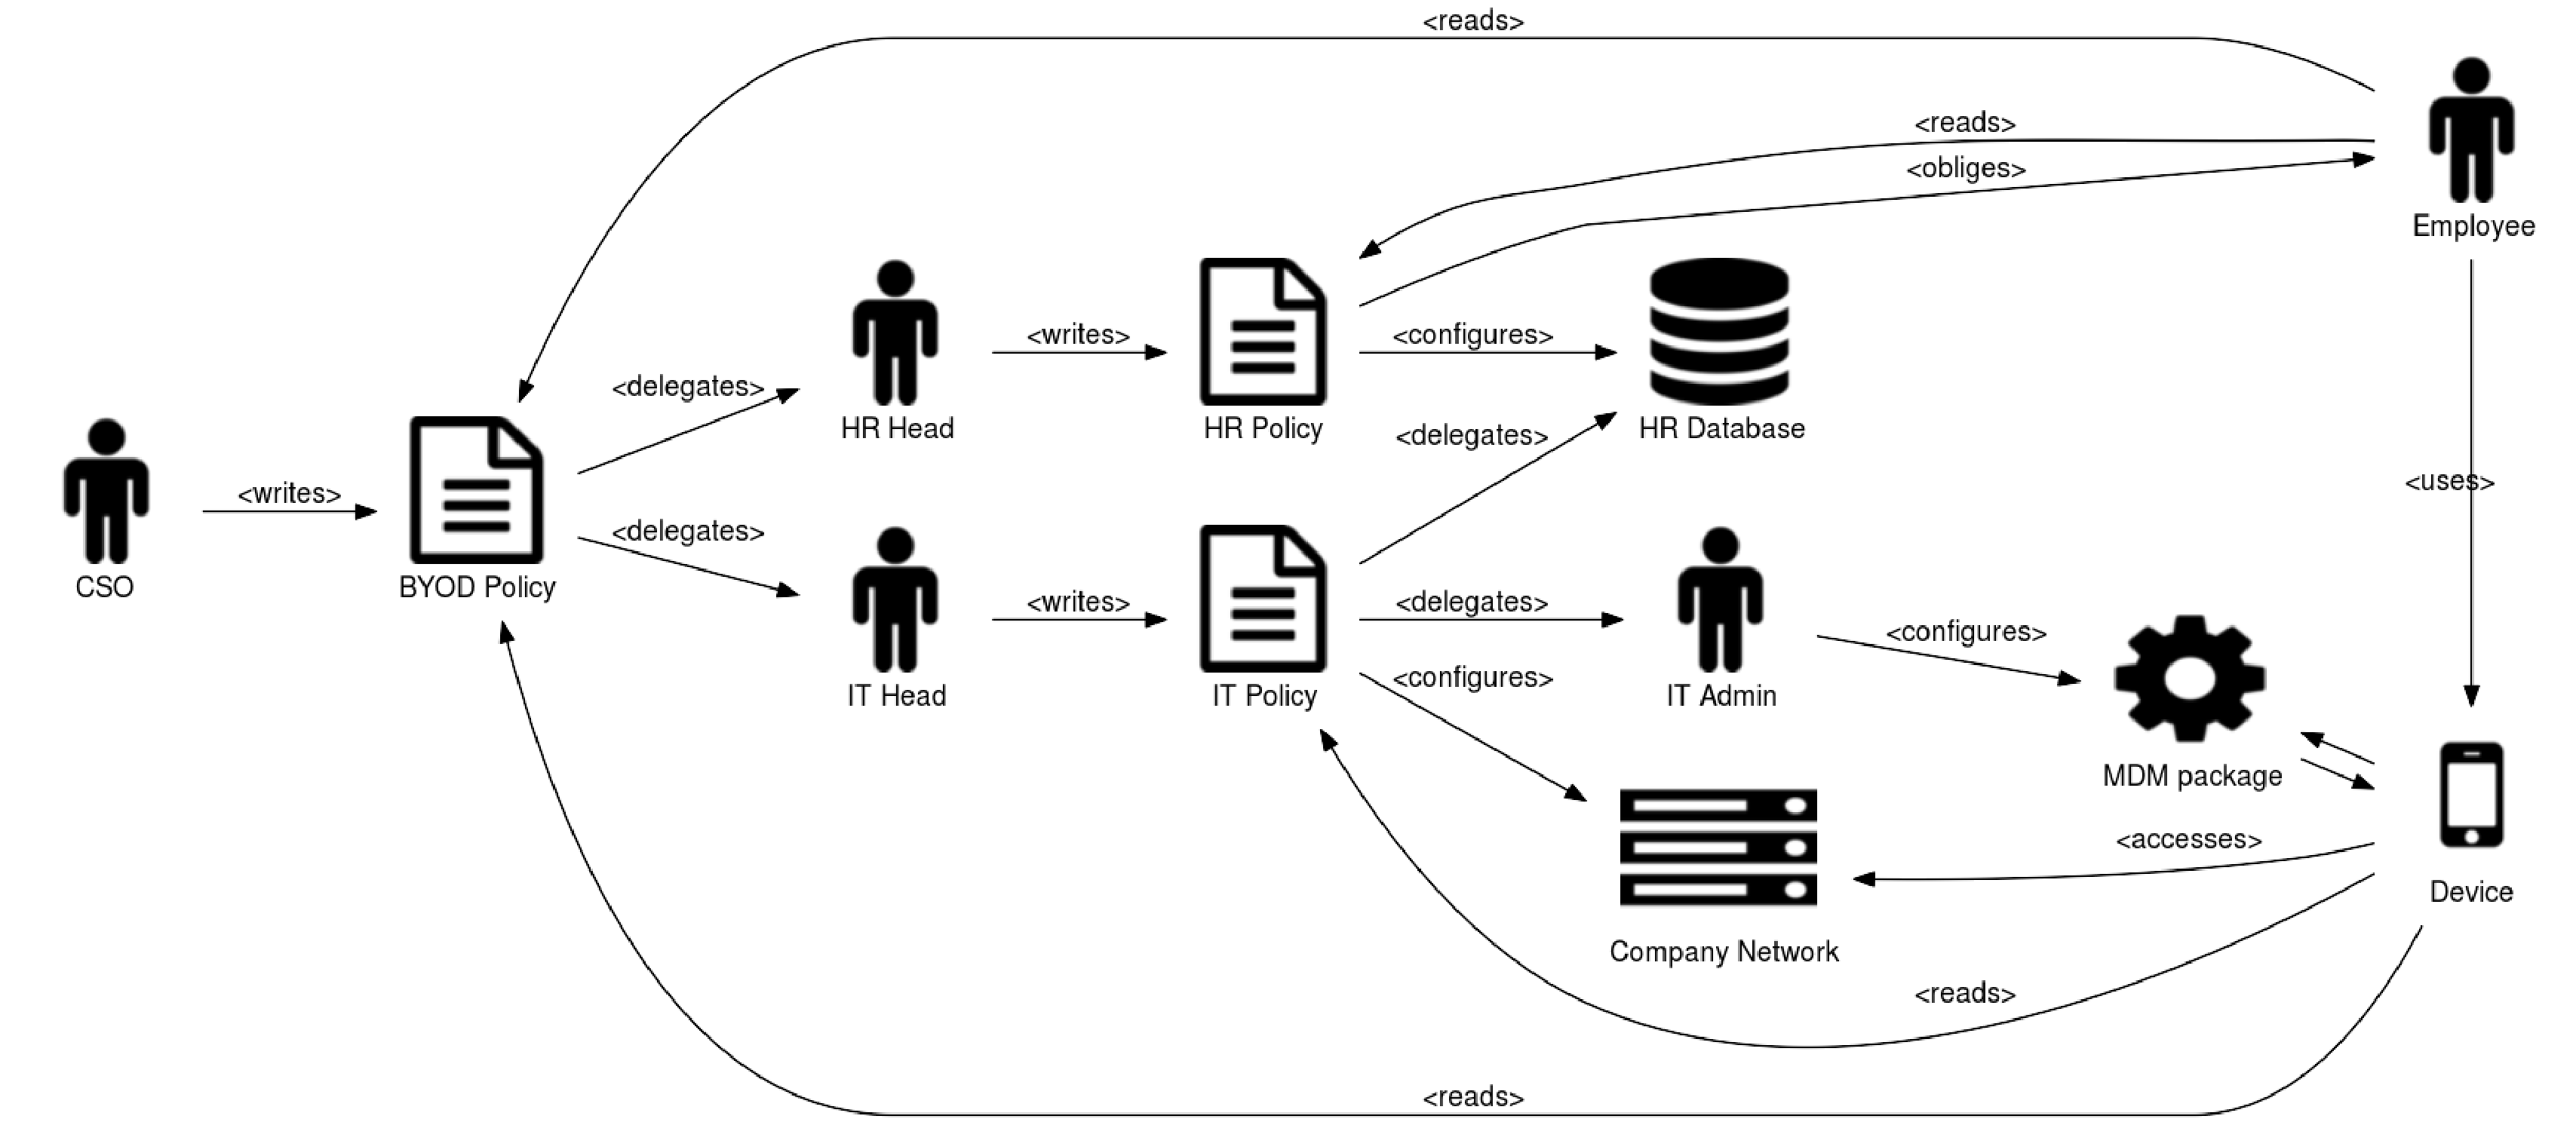
\includegraphics[width=\textwidth]{figures/mdm-overview.pdf}
  \caption{Interactions in a company with BYOD security policies.}
  \label{fig:mdm-overview}
\end{figure}

This work has so far focused on the contents of the BYOD policies.
The concerns and delegation relationships have been highlighted as
they are not handled well by existing \ac{MDM} tools.  The policies
also contain rules that the \ac{MDM} tools do manage well:
configuring, provisioning and wiping devices.  The \ac{MDM} tools
fail, however, to give a means to control \emph{how} they themselves
are configured; with the typical method being through the manual
intervention of an IT administrator.

AppPAL exists as a tool for checking whether a policy is satisfied.
It is reasonable to ask what would a company have to do to
\emph{enforce} their mobile device policies. A company could have a
structure such as in \autoref{fig:mdm-overview}: the Chief Security
Officer sets the BYOD policy, which delegates to IT and HR to further
specify parts of the policy.  Employees are obliged to read all the
policies put out and follow them (by HR).  The IT department who
maintain the company network, configure the \ac{MDM} software on the
employee's device, to ensure it meets their policies.

AppPAL offers a company the means to describe the policy precisely and
check if it satisfied; to
implement the policy the company would need to implement actions atop
of these checks.  If AppPAL checks a policy and finds a user must
install an app or disable a feature on their phone, then the company
might want to configure their \ac{MDM} software to perform the
necessary steps.  If AppPAL were to discover that an employee hadn't
satisfied the obligation to sign a contract, then the company might
want to email a reminder to the employee.

AppPAL doesn't remove the need for \ac{MDM} software.  Much of an
\ac{MDM} package's functionality could be re-implemented as part of
AppPAL, but this is an unnecessary duplication of work.  Rather AppPAL
should be used to configure other, existing tools.  An \ac{MDM}
package could enfore a password policy, and enable remote wipe (for
example).  Google's \emph{For Work} tools can enforce access control
policies for a company's documents, as can Microsoft's Office Suite.
The settings on an Android app control what permissions an app can
have.  \ac{MDM} tools provide a mechanism to control how a mobile
device behaves, and what an employee can do with a device.  Alone,
however, they do not provide enough to fully enforce a \ac{BYOD}
policy as all the \ac{BYOD} policies we examined contained more than
just device configuration.

AppPAL works as a glue between existing tools.  It tells an
administrator what configuration changes need to be made to satisfy a
policy, if these can be automated then so much the better.  In this
respect AppPAL is similar to a configuration language.  Giving
employees a means to make AppPAL statements (for example a dialog box
that says \emph{``type your password to acknowledge the following
policy.''}) lets us track what people have done and make decisions on
the basis of their actions.

%\comment{
%  \bibliography{thesis}
%}
\end{document}


%%% Local Variables:
%%% mode: latex
%%% TeX-master: "../ch5"
%%% End:
